\begin{enumerate}
\item 

\mbox{$f(10)=-\np{0.25}\times10^2+30\times10-500=-\np{0.25}\times100+300-500=-225$} : l'image de $10$ par $f$ est $-225$.
\item 

On développe \mbox{$(-\np{0.25}x+5)(x-100)=-\np{0.25}x\times x-\np{0.25}x\times(-100)+5\times x+5\times(-100)$}.

Donc  \mbox{$(-\np{0.25}x+5)(x-100)=-\np{0.25}x^2+25x+5 x-500=f(x)$}.

\mbox{$(-\np{0.25}x+5)(x-100)$} est la forme factorisée de $f(x)$.
\item 

\mbox{$f(x)=0\iff -\np{0.25}x+5=0\text{ ou }x-100=0$} (équation \og{}produit nul\fg{}).
Il y a deux solutions qui sont 20 et 100.
\item 

On a \mbox{$f'(x)=-\np{0.25}\times2x+30=-\np{0.5}x+30$}.
\item 

$f'$ est positive puis négative, et change de signe pour \mbox{$x=60$}.
$f$ est donc croissante puis décroissante, et on peut construire son tableau de variations :

\begin{center}
	\begin{adjustbox}{max width=1\linewidth,max totalheight=255mm}
	\begin{tikzpicture}[xscale=1,yscale=1,rotate=0,every node/.style={scale=1,rotate=0}]
		\tkzTabInit[deltacl=1]          {$x$/0.85,$f~'(x)$/.85,$f(x)$/2.5}
		
		{$0$,$60$,$200$}		
		\tkzTabLine{,+,0,-,}
		\tkzTabVar{-/$-500$,+/$400$,-/$-\np{4500}$}			

	\end{tikzpicture}
\end{adjustbox} 

\end{center}
\textit{NB}: vraisemblablement, les valeurs prises par $f$ ne sont pas exigibles dans le tableau de variations.

Pour $f(0)$, c'est quand même simple \dots

Pour $f(60)$, \mbox{$6\times6=36$}, donc \mbox{$60^2=\np{3600}$}, et \mbox{$-\np{0.25}\times\np{3600}=-900$} (le quart\dots)  \mbox{$3\times6=18$}, donc \mbox{$30\times60=\np{1800}$}, on a donc \og{}au final\fg{} \mbox{$f(60)=-900+\np{1800}-500=400$}.

Enfin pour \mbox{$f(200)$}, \mbox{$2^2=4$}, donc \mbox{$200^2=\np{40000}$}.

\mbox{$-\np{0.25}\times200^2=-\np{10000}$}. \mbox{$30\times200=\np{6000}$}, donc \mbox{$f(200)=-\np{10000}+\np{6000}-\np{500}=-\np{4500}$}.

\end{enumerate}
